\documentclass[12pt, draftcls, onecolumn]{IEEEtran}
\makeatletter
\def\subsubsection{\@startsection{subsubsection}
                                 {3}
                                 {\z@}
                                 {0ex plus 0.1ex minus 0.1ex}
                                 {0ex}
                                 {\normalfont\normalsize\bfseries}}
\makeatother
\usepackage[T1]{fontenc}
\usepackage{subfigure}
\usepackage{ulem}
\usepackage{amsmath}
\usepackage{hyperref}
\allowdisplaybreaks
\usepackage{hhline}
\usepackage{yfonts,color}
\usepackage{soul,xcolor}
\usepackage{verbatim}
\usepackage{amsmath}
\allowdisplaybreaks
\usepackage{amssymb}
\usepackage{amsthm}
\usepackage{float}
\usepackage{bm}
\usepackage{url}
\usepackage{array}
\usepackage{cite}
\usepackage{graphicx}
\usepackage{framed}
\usepackage{balance}
\usepackage{epsfig,epstopdf}
\usepackage{booktabs}
\usepackage{courier}
\usepackage{subfigure}
\usepackage{pseudocode}
\usepackage{enumerate}
\usepackage{algorithm}
\usepackage{algpseudocode}
\newtheorem{definition}{Definition}
\newtheorem{theorem}{Theorem}
\newtheorem{lemma}[theorem]{Lemma}
\newtheorem{proposition}[theorem]{Proposition}
\newtheorem{corollary}[theorem]{Corollary}
\newtheorem{assumption}{Assumption}
\newtheorem{remark}{Remark}
\renewcommand{\algorithmicrequire}{\textbf{Initialization:}}
\renewcommand{\algorithmicensure}{\textbf{Output:}}
\newcommand{\rom}[1]{\uppercase\expandafter{\romannumeral #1\relax}}
\usepackage{color}
\usepackage{soul,xcolor}
\newcommand{\nm}[1]{{\color{blue}\text{\bf{[NM: #1]}}}}
\newcommand{\sst}[1]{\st{#1}}
\newcommand{\gs}[1]{{\color{orange}\bf{[GS: #1]}}}
\newcommand{\remove}[1]{{\color{magenta}{\bf REMOVE: [#1]}}}
\newcommand{\add}[1]{{\color{red}{#1}}}
\newcommand{\ull}[1]{\textbf{\color{red}\ul{#1}}}
\usepackage{cleveref}
\Crefname{figure}{Fig.}{Figs.}
\normalem
\begin{document} 
\setulcolor{red}
\setul{red}{2pt}
\title{NSF POWDER Measurement Campaign\\ \Large{28 GHz Communication System Setup and Walk-through}}
\author{Bharath Keshavamurthy and Yaguang Zhang}
\maketitle
\setstcolor{red}
\section{Initial Calibrations \& Validations}\label{I}
\begin{enumerate}
    \item Before setting up the circuitry, using a multimeter, confirm that the available regulated power supplies and/or batteries (rechargeable: SLA) meet the current and voltage needs of the components in the Tx and Rx circuits. Note that the voltage and current ratings for the following components are their respective typical values for indoor tests:
    \begin{itemize}
        \item Tx WR-$28$ horn antenna and $28$GHz up-converter: $12{\pm}0.3$V, with $0.64{\pm}0.03$A;
        \item Rx WR-$28$ horn antenna and $28$GHz down-converter: $12{\pm}0.3$V, with $0.36{\pm}0.03$A;
        \item \label{step:1p} Tx and Rx PN-sequence generators: $12{\pm}0.3$V, with $0.33{\pm}0.03$A; and
        \item Tx and Rx MiniCircuits ZFL-$1000+$ amplifier: $12{\pm}0.3$V, with $50{\pm}10$mA, providing $17$dB gain at $12$V for $384.70$MHz input; Nominal DC voltage: $15$V, Maximum current: $105$mA.
    \end{itemize}
    \item After ensuring that the available power supplies and/or batteries meet the aforementioned voltage and current needs, connect the Tx and Rx horn antennas and their associated $28$GHz up/down converters to their corresponding power supplies. Make sure that the power supplies and/or batteries have been turned OFF before continuing on to the next step.
    \item Next, confirm that the bare-bones/stripped-down $28$GHz communication (up-converted at $2.5$GHz at the Tx and down-converted to $2.5$GHz at the Rx) works as expected between the Tx WR-$28$ horn antenna (with its $28$GHz up-converter) and the Rx WR-$28$ horn antenna (with its $28$GHz down-converter):
    \begin{itemize}
        \item Connect a signal generator to the input channel of the Tx-side up-converter \texttt{-{}-} make sure that the signal generator has "RF OFF" and "MOD OFF", and set the output frequency of the signal generator to $2.5$GHz \& its signal amplitude to $-50$dBm;
        \item Connect the output channel of the Rx-side down-converter to a spectrum analyzer, with the analyzer configured to a center frequency of $2.5$GHz \& a span of $100$kHz;
        \item Ensure that the Tx and Rx antennas are reasonably aligned with each other;
        \item Turn on the Tx and Rx power supplies and/or batteries, turn "RF ON" on the signal generator, and observe the output on the spectrum analyzer \texttt{-{}-} which should appear as depicted in Fig. \ref{fig:1};
        \begin{figure}
            \centering
            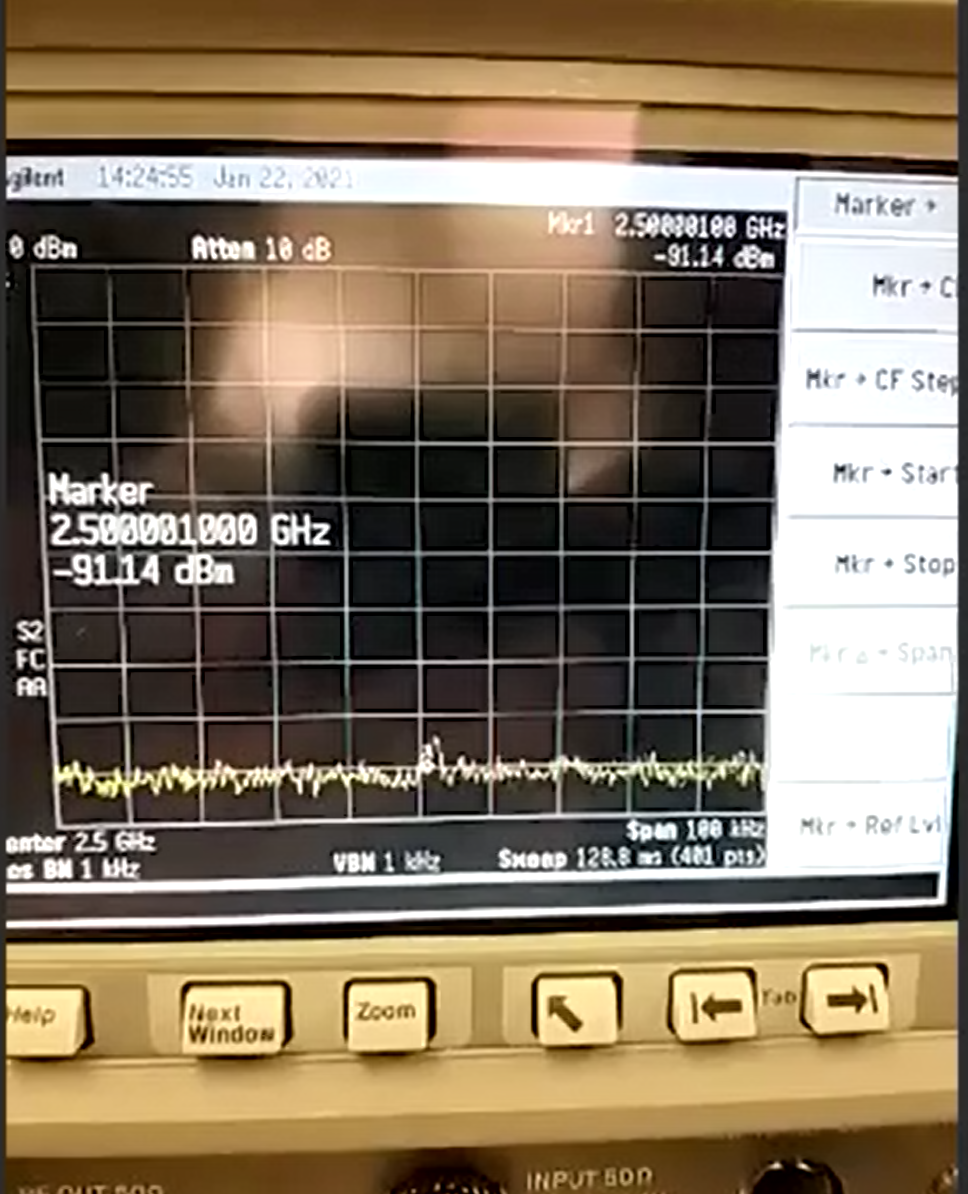
\includegraphics[width=15cm, height=12.5cm]{1.png}
            \caption{The $2.5$GHz down-converted output from the Rx WR-$28$ horn-antenna and its $28$GHz down-converter, as observed on an Agilent E-series spectrum analyzer}
            \label{fig:1}
        \end{figure}
        \item With the connections and configurations in place, increase the signal amplitude at the signal generator to $-40$dBm and observe an increase in the amplitude of the down-converted signal on the analyzer \texttt{-{}-} as depicted in Fig. \ref{fig:2};
        \begin{figure}
            \centering
            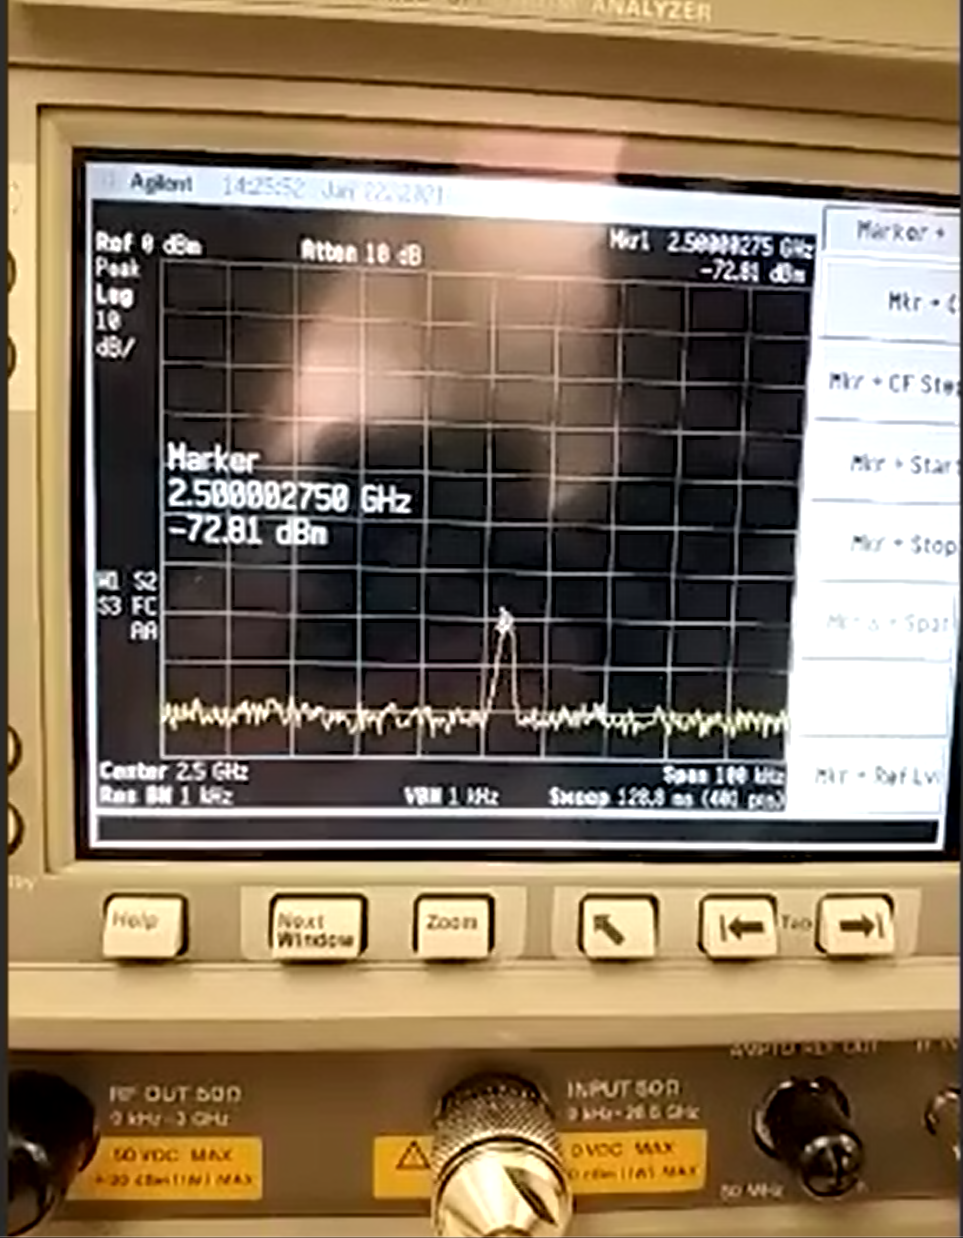
\includegraphics[width=15cm, height=12.5cm]{2.png}
            \caption{An increase in the amplitude of the $2.5$GHz down-converted output from the Rx WR-$28$ horn-antenna and its $28$GHz down-converter \texttt{-{}-} when the signal amplitude at the Tx-side signal generator is increased to $-40$dBm, as observed on an Agilent E-series spectrum analyzer}
            \label{fig:2}
        \end{figure}
        \item Set "RF OFF" on the signal generator, and turn OFF the power-supplies and/or batteries at the Tx and Rx ends to set things up for the next phase of calibrations \& validations; and note the following warning on the input signal amplitude to the Tx system from the signal generator.
        \item \textcolor{red}{WARNING: The maximum signal amplitude the Tx-side antenna and up-converter system can handle is $-4$dBm. In indoor settings, it is recommended to limit this signal amplitude to $-30$dBm.} 
    \end{itemize}
    \item Next, confirm that both the Tx and Rx side PN-sequence generators operate as expected by executing the following steps for the two:
    \begin{itemize}
        \item Connect the output channel of the signal generator to the input channel of the PN-sequence generator (CLK), with its frequency set to $50$MHz and its amplitude set to $0$dBm; note here that these PN sequence generators can handle input signal amplitudes in the range of $-10$dBm to $10$dBm; Ensure that RF is OFF on the signal generator;
        \item Connect the PN-sequence generator to its corresponding power-supply or battery (based on the voltage and current ratings mentioned in step \ref{step:1p}); Make sure that the power supply or the battery is turned OFF;
        \item Connect the output channel of the PN-sequence generator to the spectrum analyzer, with the analyzer's start frequency set to $0$Hz and its stop frequency set to $500$MHz;
        \item Turn ON the power-supply or battery, turn RF ON on the signal generator, toggle the run-stop switch on the PN-sequence generator, and observe the PN-sequence generator's output on the spectrum analyzer \texttt{-{}-} which should appear as depicted in Fig. \ref{fig:3}, i.e., a sinc-squared waveform with its nulls located at integer multiples of the CLK frequency (50 MHz); and
        \begin{figure}
            \centering
            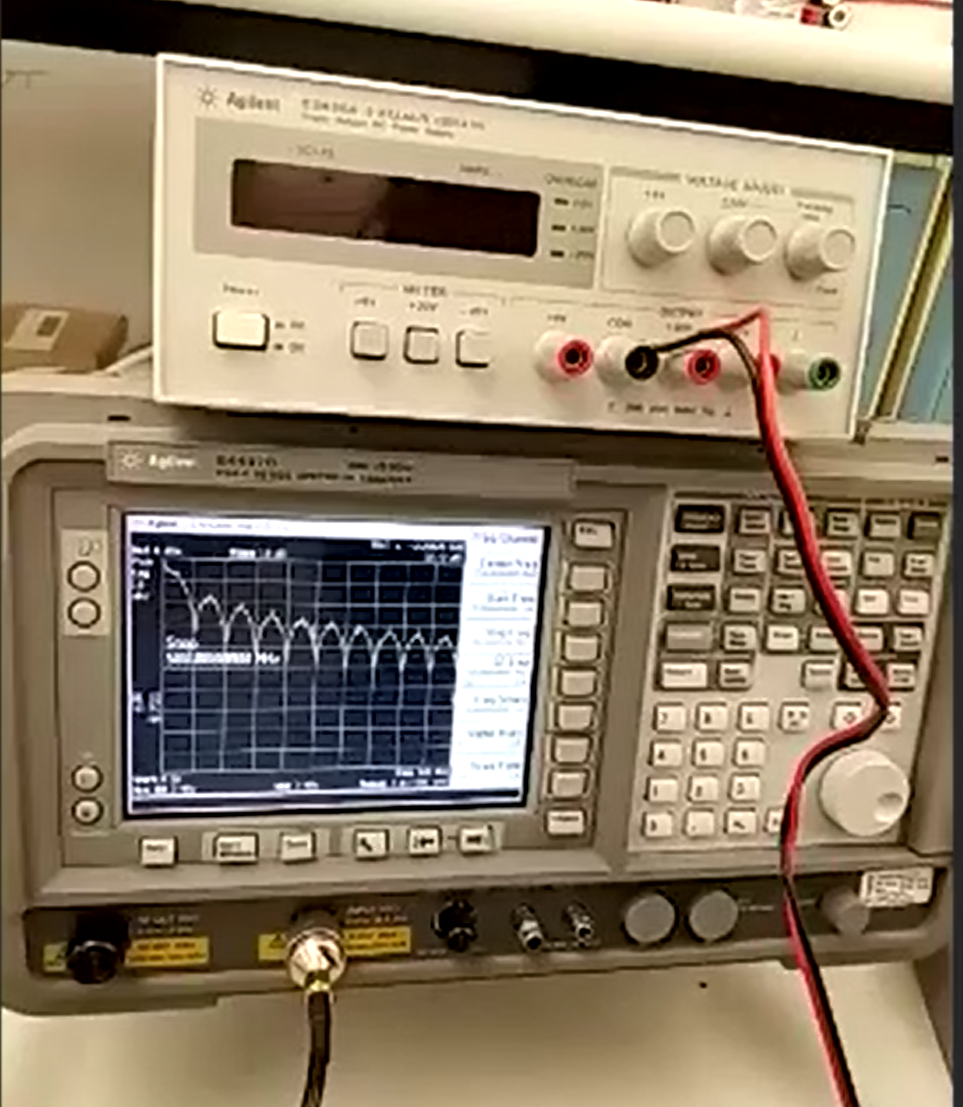
\includegraphics[width=15cm, height=12.5cm]{3.png}
            \caption{The output of the PN-sequence generator in relation to a CLK input of ($50$MHz, $0$dBm), as observed on an Agilent E-series spectrum analyzer: the first null is at $50$MHz}
            \label{fig:3}
        \end{figure}
        \item To validate the operations of the PN-sequence generator further, with the connections and configurations intact, change the frequency at the signal generator to $400$MHz, toggle the run-stop switch on the PN-sequence generator, and observe the PN-sequence generator's output on the spectrum analyzer \texttt{-{}-} which should appear as depicted in Fig. \ref{fig:4}, i.e., a sinc-squared waveform with its nulls located at integer multiples of the CLK frequency (400 MHz).
        \begin{figure}
            \centering
            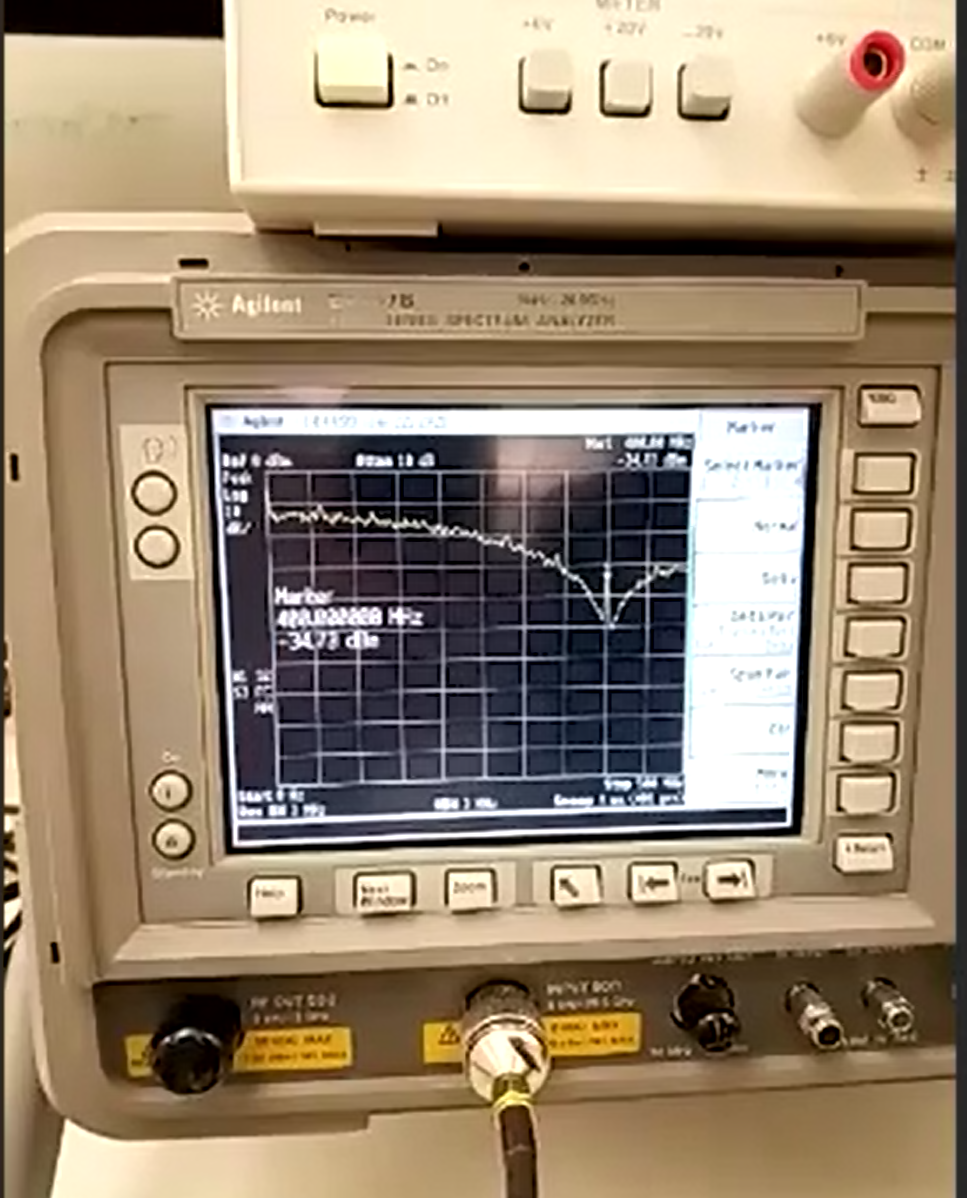
\includegraphics[width=15cm, height=12.5cm]{4.png}
            \caption{The output of the PN-sequence generator in relation to a CLK input of ($400$MHz, $0$dBm), as observed on an Agilent E-series spectrum analyzer: the first null is at $400$MHz}
            \label{fig:4}
        \end{figure}
    \end{itemize}
    \item \textcolor{blue}{DEBUG: If a PN-sequence generator does not work as detailed above, execute the following steps to debug the problem, breaking-off of the point at which the debug step fails to meet expectations to fix the issue \texttt{-{}-} which might include re-soldering components on the circuit board: 
    \begin{itemize}
        \item Set "RF OFF" on the signal generator, keep the connections intact, and the power-supply/battery turned ON;
        \item To ensure that the PN-sequence generator is being powered correctly, use a multimeter to measure the voltage between the GND strip and the tap of the voltage regulator \texttt{-{}-} which should be $5{\pm}0.3$V;
        \item To ensure that the run-stop toggle switch on the PN-sequence generator is operating correctly, with the switch set to STOP, use a multimeter to measure the voltage between the GND strip and the point identified by a red circle in Fig. \ref{fig:5} \texttt{-{}-} the multimeter should read $4{\pm}0.3$V; and with the switch set to RUN, the voltage between the same two points should be $3{\pm}0.3$V;
        \begin{figure}
            \centering
            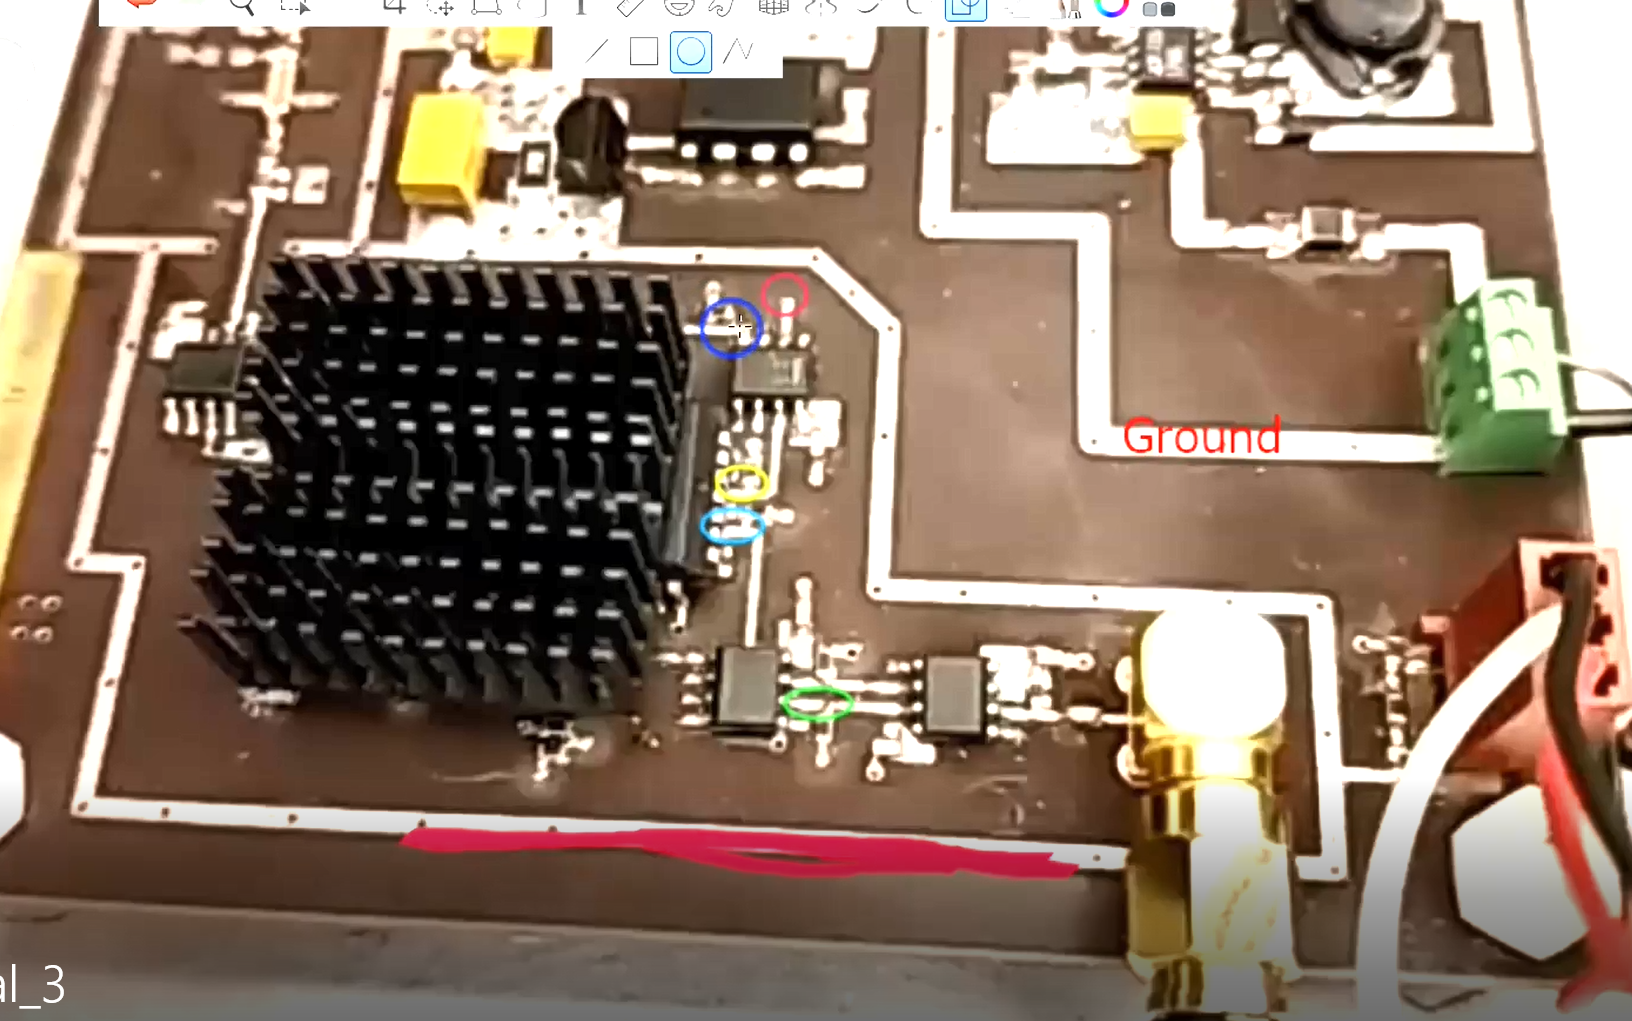
\includegraphics[width=15cm, height=10cm]{12.png}
            \caption{The set of debug points on the PN-sequence generator's circuit board}
            \label{fig:5}
        \end{figure}
        \item \label{step:debug-o-1} To check if a $10$MHz square waveform is propagating through the PN sequence generator at the point highlighted by a green oval in Fig. \ref{fig:5}, place a probe of an oscilloscope at this point and the other probe on the strip highlighted by a bold red line in Fig. \ref{fig:5} \texttt{-{}-} the $10$MHz square waveform should appear on the oscilloscope as depicted in Fig. \ref{fig:6} (a horizontal [time] scale zoom-in might be needed to get a good view of the waveform on the oscilloscope); and
        \begin{figure}
            \centering
            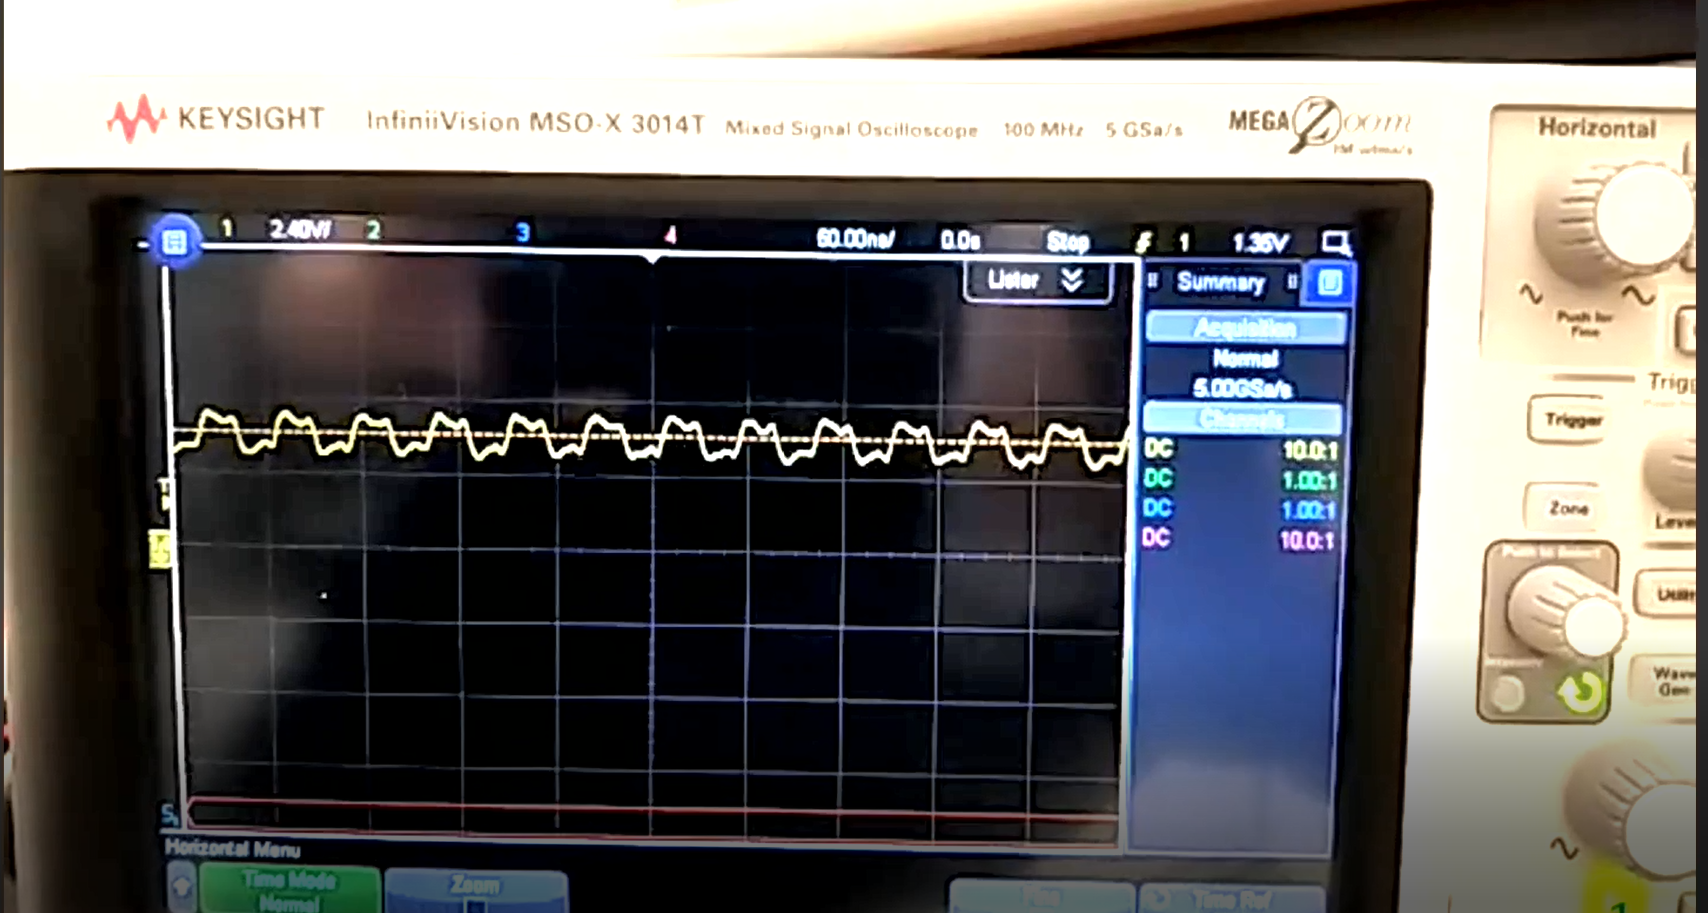
\includegraphics[width=15cm, height=10cm]{10.png}
            \caption{The $10$MHz square waveform as seen on a Keysight mixed-signal oscilloscope, when the PN-sequence generator is probed according to the procedure outlined in step \ref{step:debug-o-1}}
            \label{fig:6}
       \end{figure}
       \item \label{step:debug-o-2} As a final debug step, probe the signal between the point identified by a blue circle and the strip highlighted by a bold red line in Fig. \ref{fig:5} \texttt{-{}-} the observed waveform on the oscilloscope should be another $10$MHz square waveform as depicted in Fig. \ref{fig:7}; note here that in order to optimally observe this waveform, the oscilloscope might need to be "Edge Triggered" with a "Line Source" \texttt{-{}-} along with a vertical scale resolution of $1$V per division and a horizontal scale resolution of $20\mu$s per division.
       \begin{figure}
            \centering
            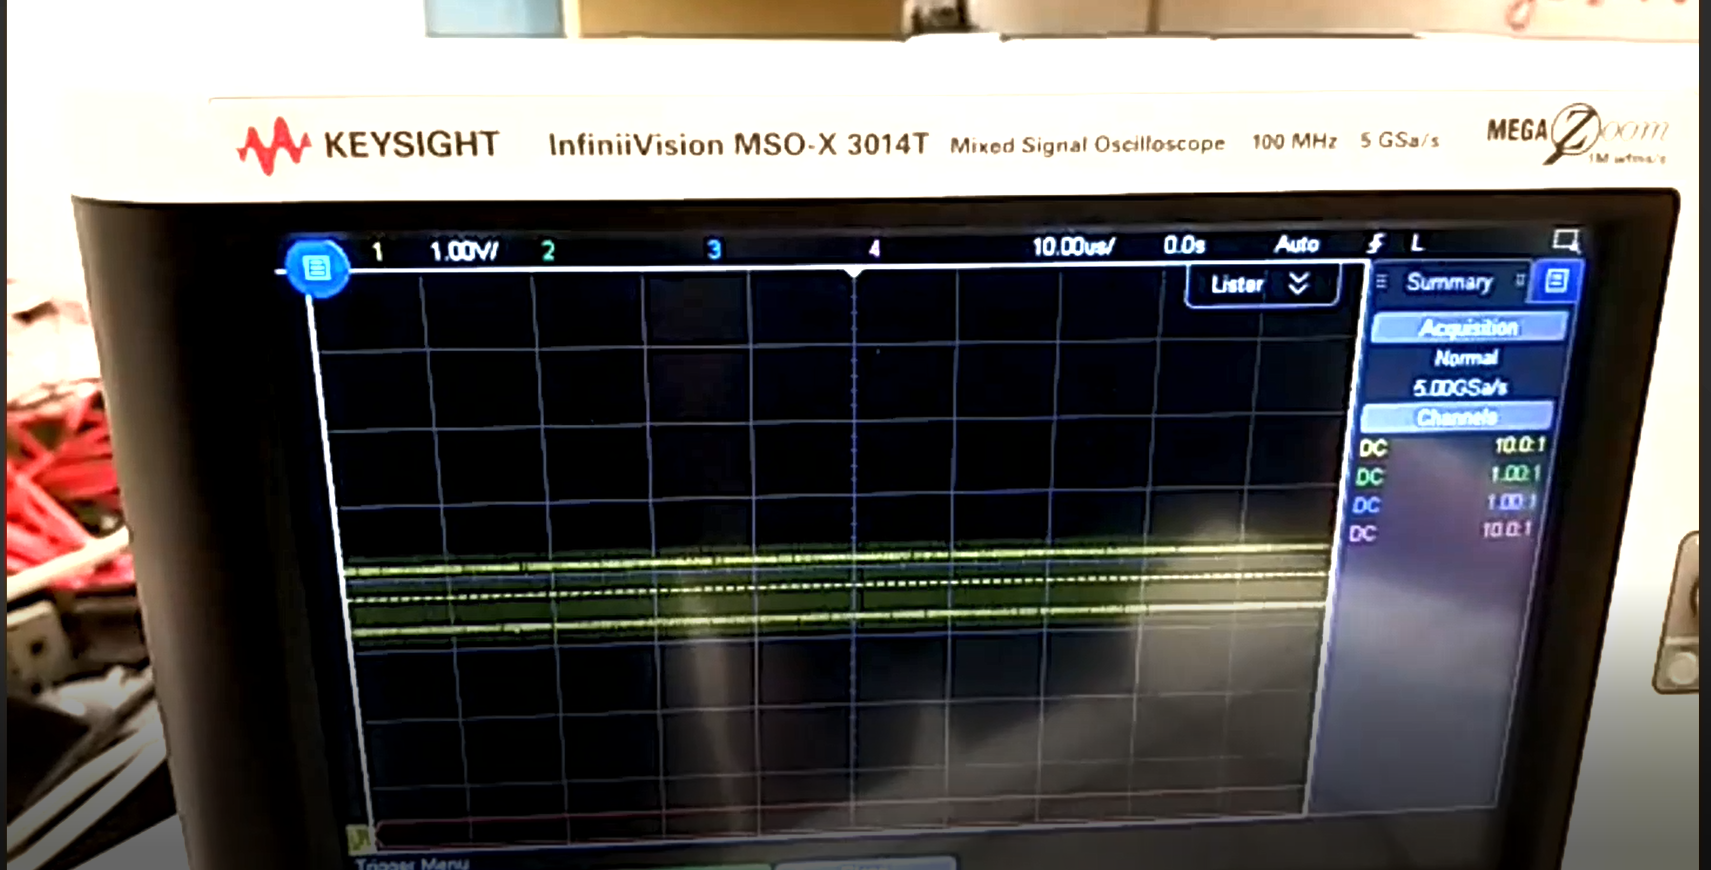
\includegraphics[width=15cm, height=10cm]{13.png}
            \caption{The $10$MHz square waveform as seen on a Keysight mixed-signal oscilloscope, when the PN-sequence generator is probed according to the procedure outlined in step \ref{step:debug-o-2}}
            \label{fig:7}
       \end{figure}
    \end{itemize}}
\end{enumerate}
\section{Complete Tx Communication System Setup \& Stripped-down Rx Validation}
\begin{enumerate}
    \item The block diagram for the Tx communication system is illustrated in Fig. \ref{fig:8}.
    \begin{figure}
        \centering
        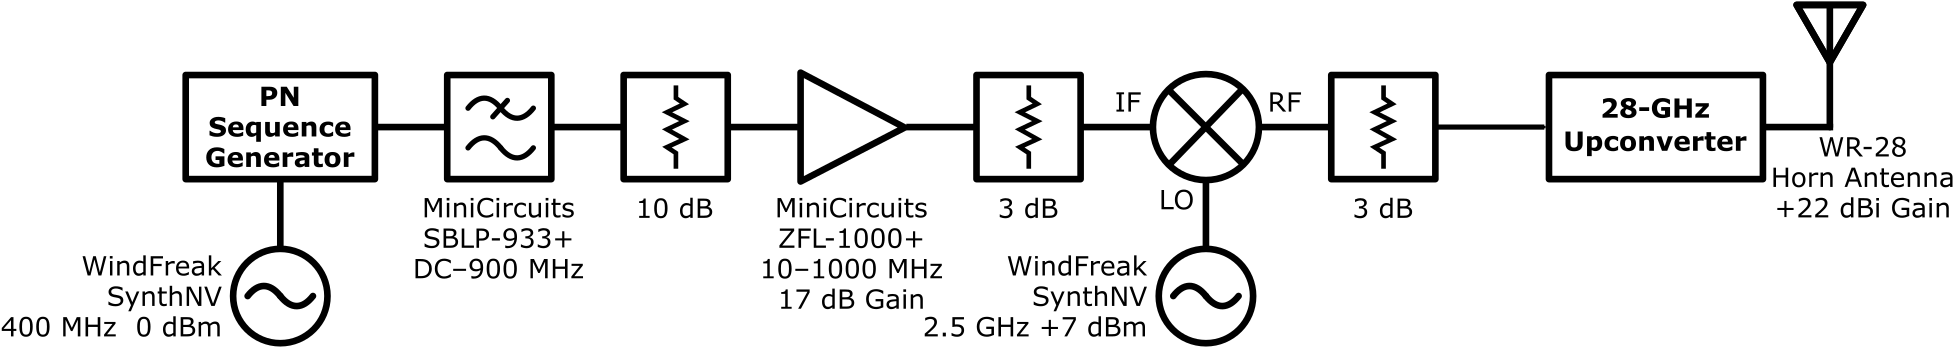
\includegraphics[width=1.0\linewidth]{14.png}
        \caption{The block-diagram of the $28$GHz Tx communication system}
        \label{fig:8}
    \end{figure}
    \item Before setting up and configuring the components in this Tx-side circuit, verify that the WindFreak frequency synthesizers (x2) used here provide the PN-sequence generator CLK signal and the LO signal at the required frequencies and amplitudes:
    \begin{itemize}
        \item For the WindFreak frequency synthesizer designated to provide the PN-sequence generator CLK, power it using a USB battery bank and connect its "RFout" port to a spectrum analyzer (start frequency set to $0$Hz, stop frequency set to $1$GHz), and observe a $400$MHz $0$dBm signal on the spectrum analyzer;
        \item For the WindFreak frequency synthesizer designated to provide the LO signal, power it using a USB battery bank and connect its "RFout" port to a spectrum analyzer (start frequency set to $0$Hz, stop frequency set to $5$GHz), and observe a $2.5$GHz $7$dBm signal on the spectrum analyzer; and
        \item If the WindFreak frequency synthesizers do not provide the correct outputs, configure their output frequencies and amplitudes via the provided Windows PC application.
    \end{itemize}
    \item With the CLK and LO signal validations complete, start connecting the components in the Tx circuit as illustrated in Fig. \ref{fig:8}, without the $28$GHz up-converter and the WR-$28$ horn antenna in the circuit; instead, connect the output of the $3$dB attenuator (the one past the mixer) to the input channel of a spectrum analyzer. Also, make sure that the power supplies and/or batteries serving the various components have been turned OFF while these connections are being made. Refer to step \ref{step:1p} for instructions on how to choose the appropriate power supplies and/or batteries for the various components involved in this circuit.
    \item An additional setup note here is that while configuring this circuit in indoor settings an additional $17$dB attenuation is recommended (but, not absolutely necessary) to be provided at the output of the existing $3$dB attenuator past the mixer in Fig. \ref{fig:8}.
    \item Turn ON all the relevant power supplies and/or batteries \texttt{-{}-} including those corresponding to the WindFreak frequency synthesizers \texttt{-{}-} while noting the current being drawn by these components in order to make sure that the power supplies and/or batteries have not been overloaded. Toggle the PN-sequence generator's run-stop switch. Set the spectrum analyzer frequency to $2.5$GHz and its span to $1.6$GHz. The signal observed on the analyzer screen is depicted in Fig. \ref{fig:9}: the main lobe should be $800$MHz wide ($-55$dBm at $2.1$GHz, $-16$dBm at $2.5$GHz [peak], and $-55$dBm at $2.9$GHz).
    \begin{figure}
        \centering
        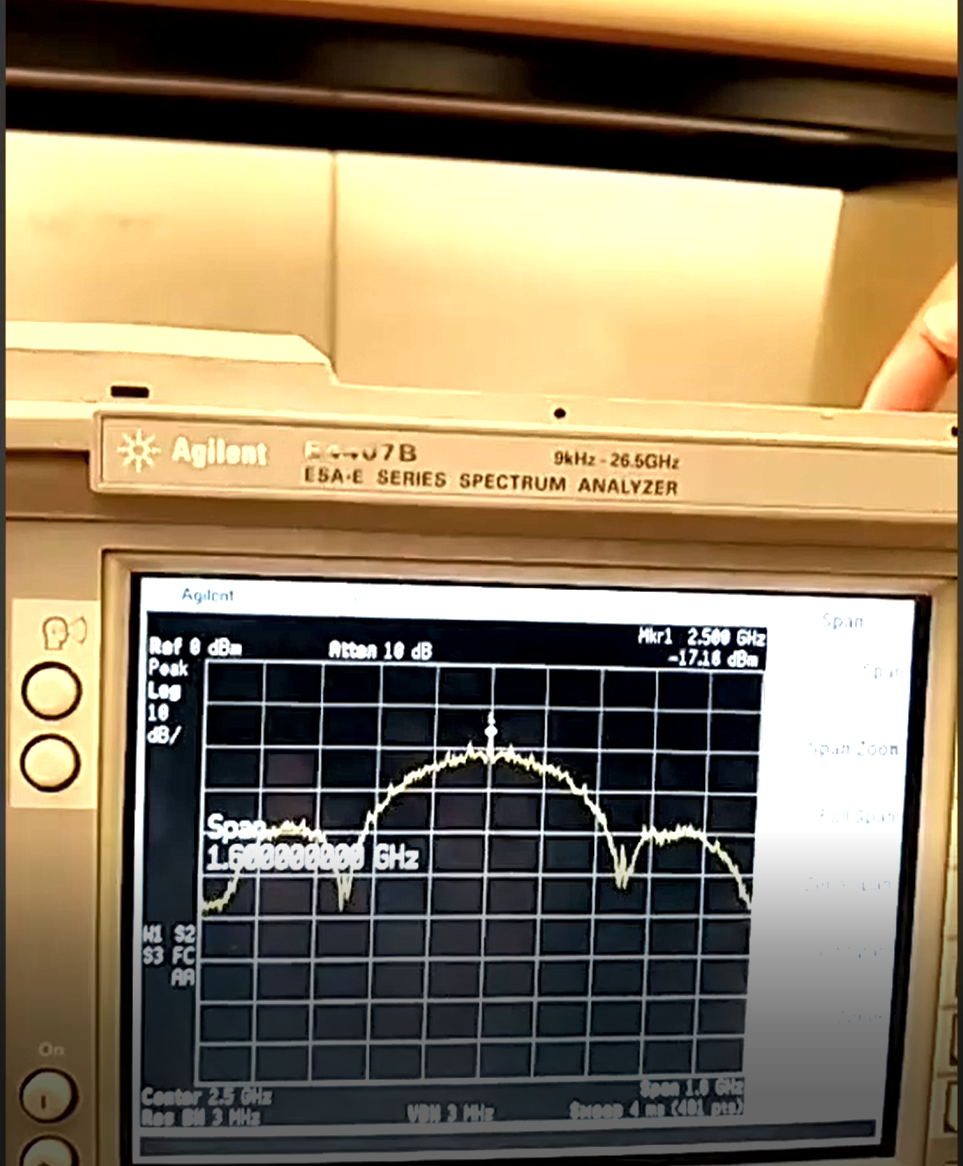
\includegraphics[width=15cm, height=12.5cm]{5.png}
        \caption{The signal observed at the input of the $28$GHz up-converter in the Tx circuit \texttt{-{}-} with $3$dB of attenuation past the mixer \texttt{-{}-} in indoor settings, as observed on an Agilent E-series spectrum analyzer}
        \label{fig:9}
    \end{figure}
    \item Now that the PN-sequence generator and the MiniCircuits associated with the Tx have been verified to be working correctly, power down all the components, and complete the circuit by connecting the output of the $3$dB attenuator to the $28$GHz up-converter.
    \item Next, in order to validate the transmitted signal reception at the Rx (bare-bones/stripped-down version), connect the output of the $28$GHz down-converter to the spectrum analyzer. Power the Rx antenna and down-converter system according to the power-supply or battery configurations laid down in \ref{step:1p}. Turn ON all the relevant power-supplies and/or batteries in the Tx circuit \texttt{-{}-} along with those corresponding to the WindFreak frequency synthesizers. Toggle the run-stop switch on the PN-sequence generator. The signal received at the output of the $28$GHz down-converter of the stripped-down Rx circuit is depicted in Fig. \ref{fig:10}: the main lobe should be $800$MHz wide ($-55$dBm at $2.1$GHz, $-16$dBm at $2.5$GHz [peak], and $-55$dBm at $2.9$GHz).
    \begin{figure}
        \centering
        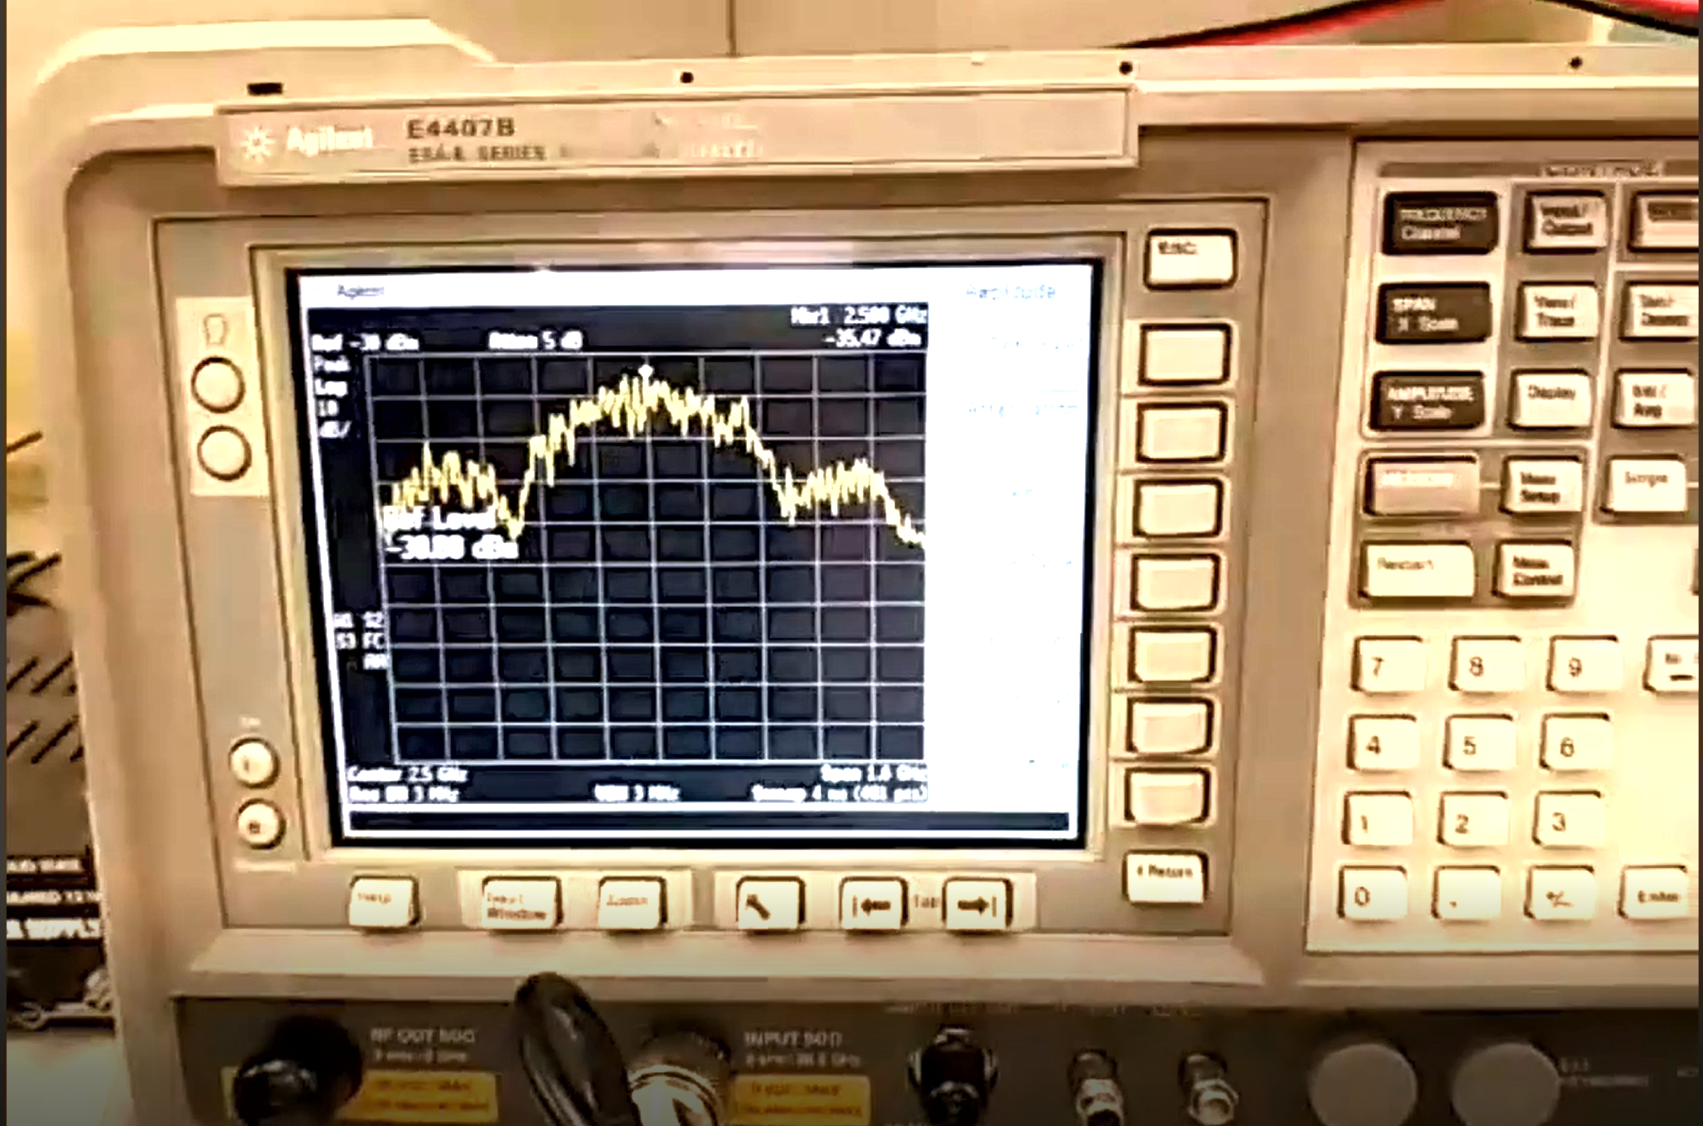
\includegraphics[width=15cm, height=12.5cm]{6.png}
        \caption{The signal observed at the output of the $28$GHz down-converter in the stripped-down Rx circuit \texttt{-{}-} with $3$dB of attenuation past the mixer in the Tx circuit \texttt{-{}-} in indoor settings, as observed on an Agilent E-series spectrum analyzer}
        \label{fig:10}
    \end{figure}
\end{enumerate}
\section{Complete Rx Communication System Setup \& Integrated Tests}
\begin{enumerate}
    \item Ensure that the power-supplies and/or batteries serving the various components in the Tx circuit have been turned OFF.
    \item The block diagram for the Rx communication system is illustrated in Fig. \ref{fig:11}.
    \begin{figure}
        \centering
        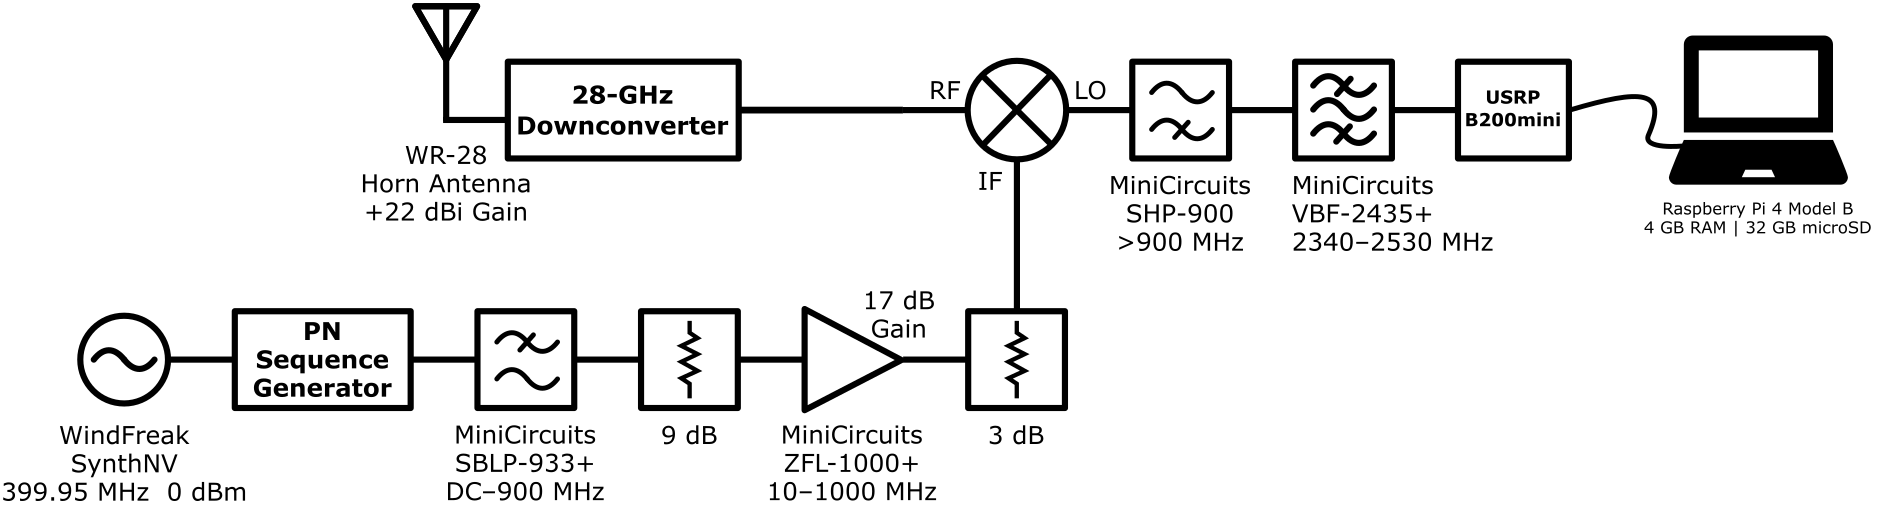
\includegraphics[width=1.0\linewidth]{15_m.png}
        \caption{The block-diagram of the $28$GHz Rx communication system}
        \label{fig:11}
    \end{figure}
    \item Before setting up and configuring the components in this Rx-side circuit, verify that the WindFreak frequency synthesizer (x1) used here provides the PN-sequence generator CLK signal at the required frequency and amplitude:
    \begin{itemize}
        \item Power this WindFreak frequency synthesizer using a USB battery bank and connect its "RFout" port to a spectrum analyzer (start frequency set to $0$Hz, stop frequency set to $1$GHz), and observe a $399.95$MHz $0$dBm signal on the spectrum analyzer \texttt{-{}-} as depicted in Fig. \ref{fig:12}.
        \begin{figure}
        \centering
        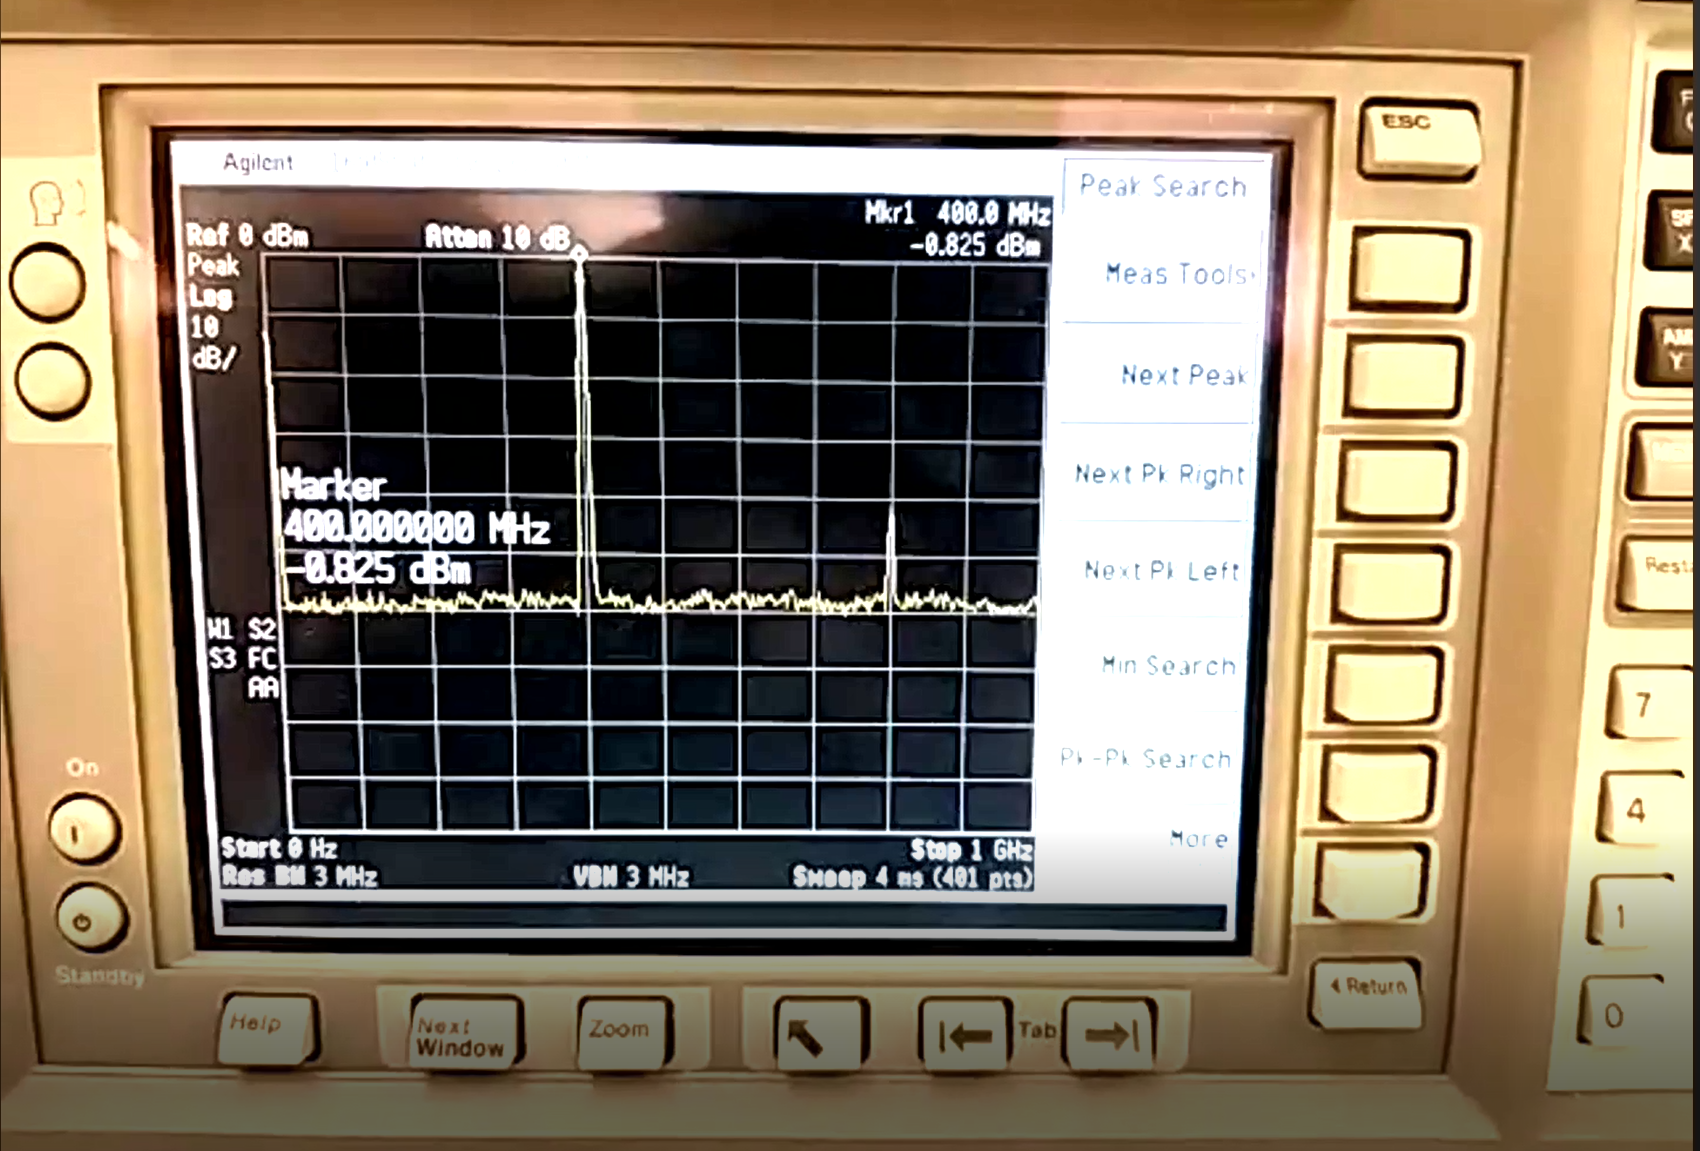
\includegraphics[width=15cm, height=12.5cm]{8.png}
        \caption{The $399.95$MHz $0$dBm CLK signal generated by the WindFreak frequency synthesizer, fed in as the reference signal to the PN-sequence generator at the Rx}
        \label{fig:12}
    \end{figure}
    \end{itemize}
    \item With the CLK signal validation complete, start connecting the components in the Rx circuit as illustrated in Fig. \ref{fig:11}. Leaving out the USRP B200mini and the Raspberry Pi, connect the output of the MiniCircuits VBF-2435+ band-pass filter to the spectrum analyzer. Ensure that the power supplies and/or batteries serving the various components have been turned OFF while these connections are being made. Refer to step \ref{step:1p} for instructions on how to choose the appropriate power supplies and/or batteries for the various components involved in this circuit.
    \item In both the Tx and Rx circuits, turn ON all the relevant power supplies and/or batteries \texttt{-{}-} including the ones corresponding to the WindFreak frequency synthesizers \texttt{-{}-} while noting the current being drawn by these components in order to make sure that the power supplies and/or batteries have not been overloaded. In both these circuits, toggle the PN-sequence generators' run-stop switch. Set the spectrum analyzer frequency to $2.5$GHz, span to $0$Hz, sweep time to $10$ms, and resolution bandwidth to $100$kHz. The signal observed on the analyzer screen is depicted in Fig. \ref{fig:13}: this corresponds to the envelope of the received signal at $2.5$GHz swept in time over a period of $10$ms per instrument reading.
    \begin{figure}
        \centering
        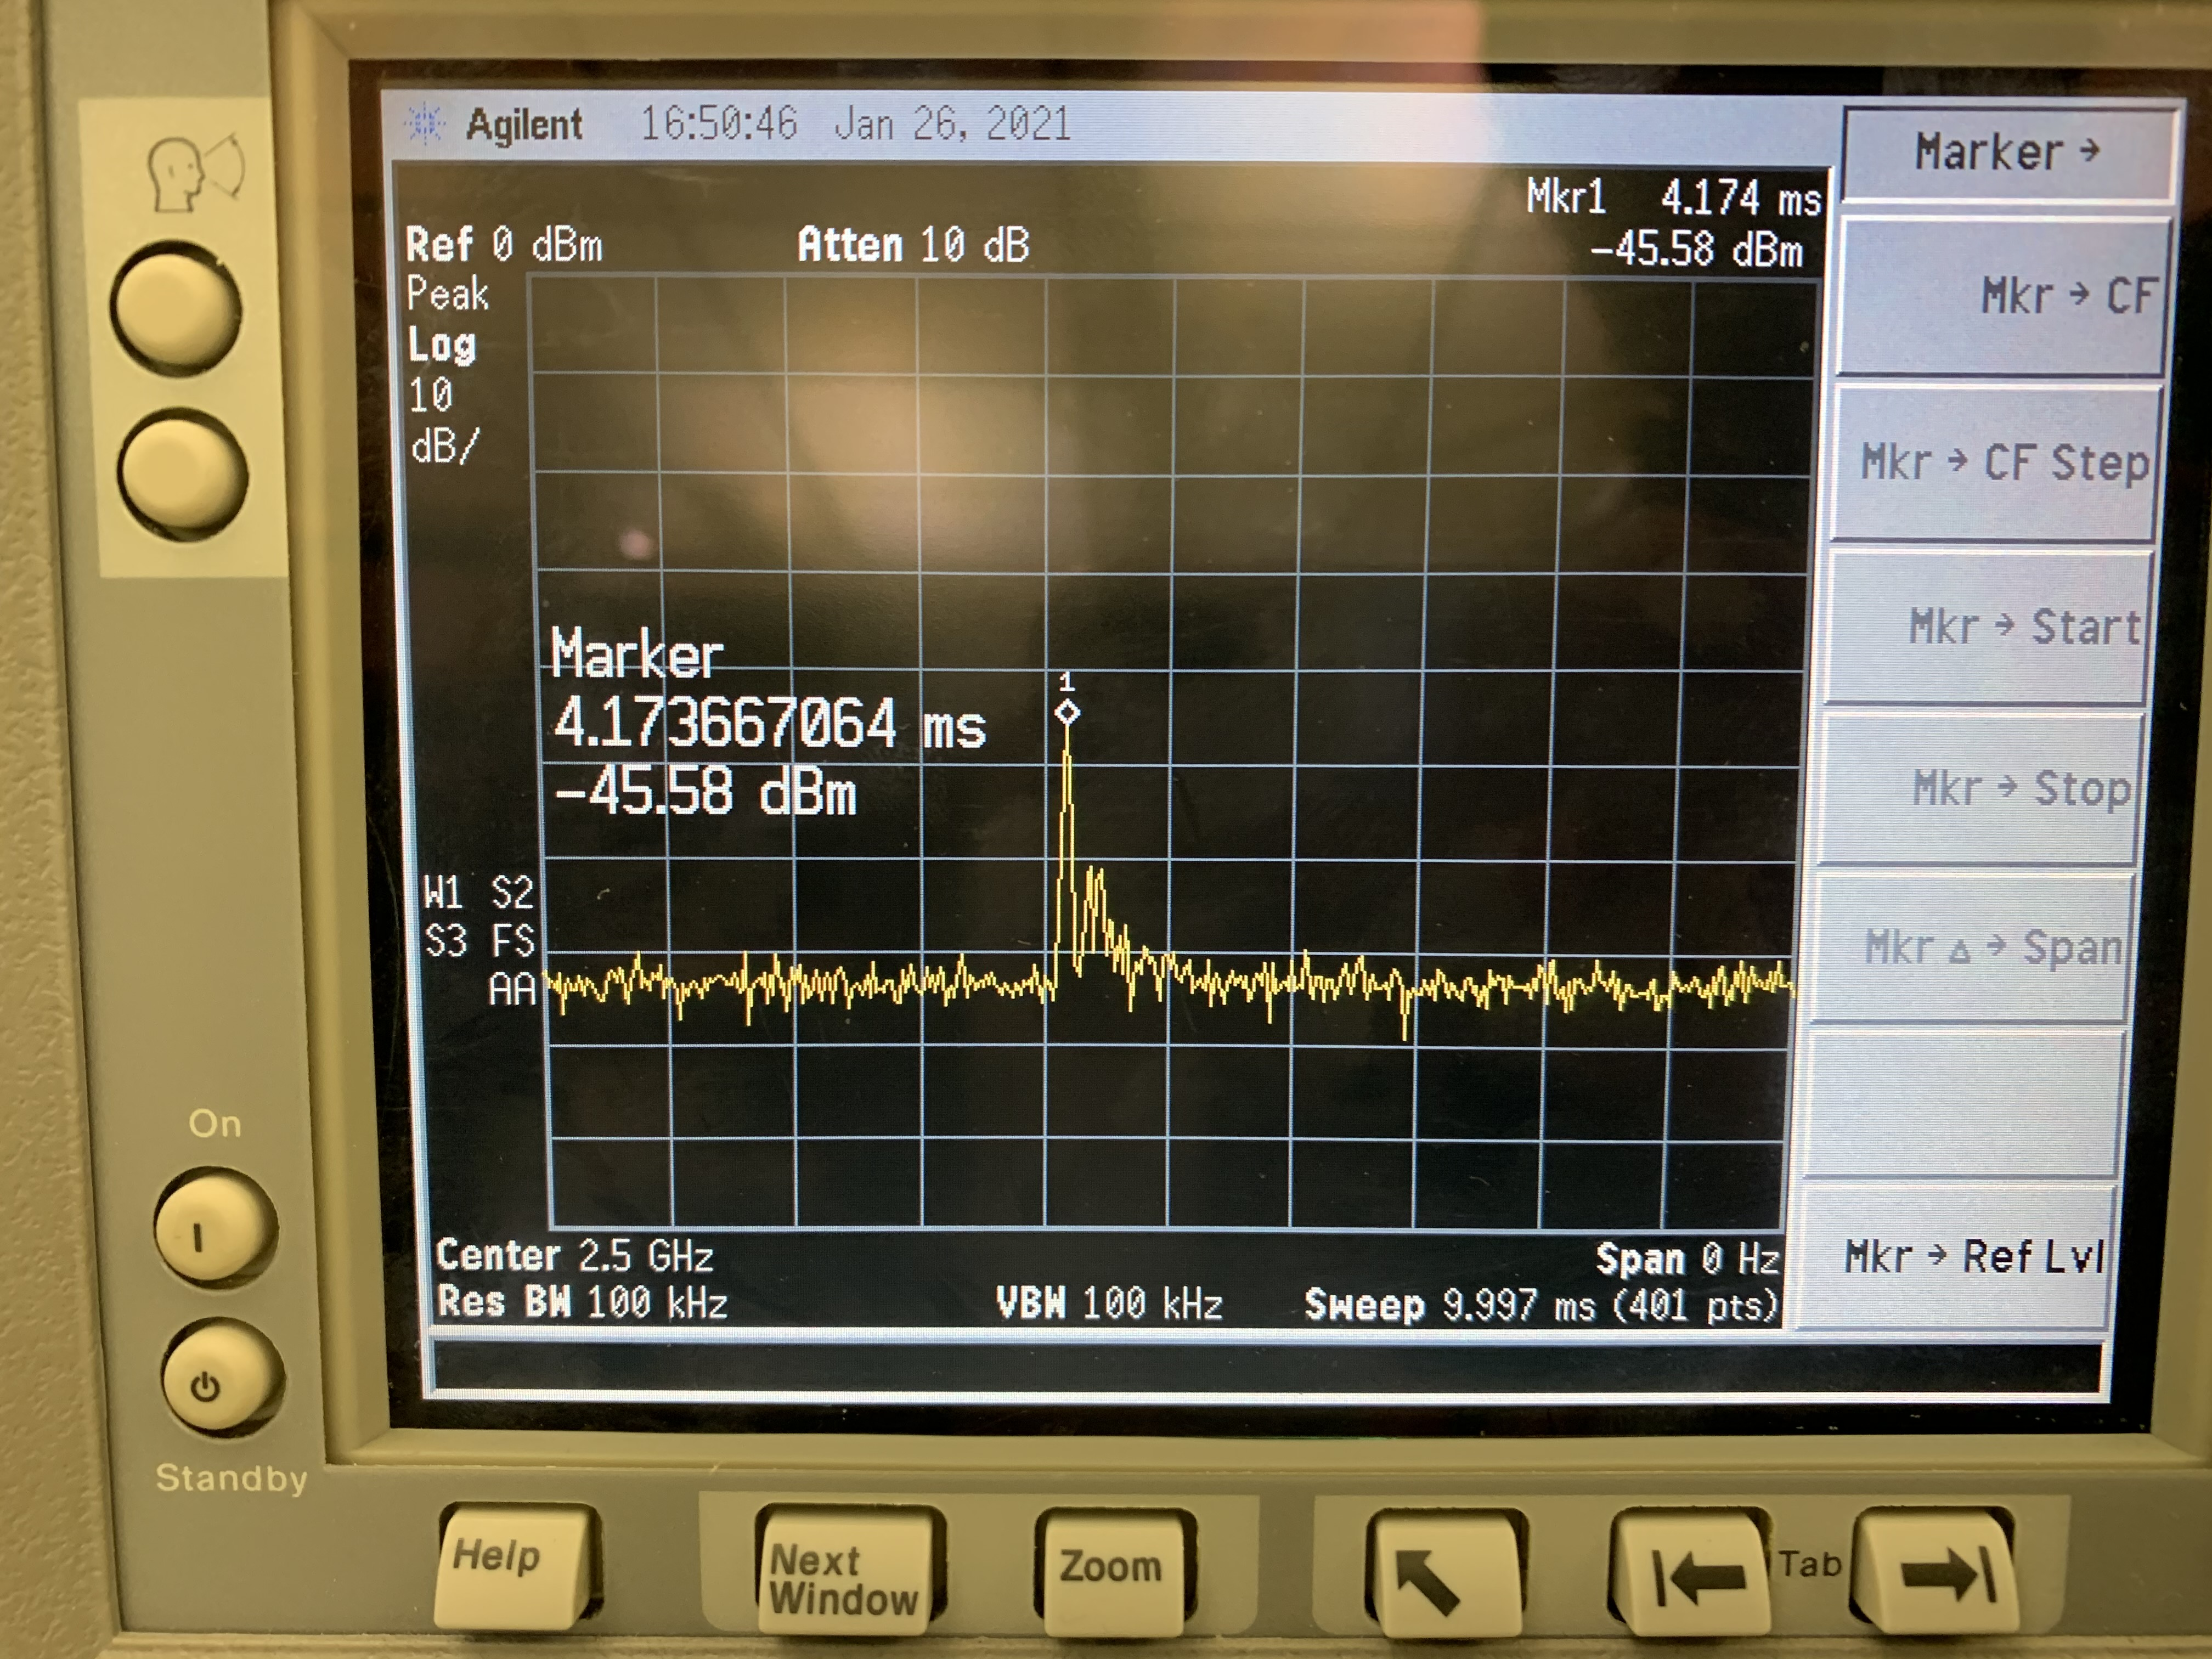
\includegraphics[width=15cm, height=12.5cm]{16.jpg}
        \caption{The power delay profile observed on an Agilent E-series spectrum analyzer: this corresponds to the envelope of the received signal at $2.5$GHz swept in time over a period of $10$ms per instrument reading; note the discernible LoS and NLoS (multi-path) components in this power delay profile}
        \label{fig:13}
    \end{figure}
    \item As a final step, these power delay profile samples need to viewed on a GNURadio scope on the Raspberry Pi through the USRP B200mini, in addition to being logged in the file-system of the Raspberry Pi, i.e., on to the available $32$GB microSD card.
\end{enumerate}

\section{Calibration for Rx Power Computation}
\label{sec_calibration}

\subsection{Overview}
After the system is set up for the measurement campaign, a calibration procedure needs to be carried out for the Rx to build a relationship between the USRP voltage readings in V and the measurement system received signal power in dB. This procedure will ensure accurate Rx power outputs with the presence of imperfect components, e.g., cables with non-negligible attenuation. Note that the Rx system in the calibration must be exactly the same as that for the measurement campaign; i.e., separate calibration is needed for each different Rx or Rx setup, even if there is only a cable replacement. 

The key calibration result: a linear relationship between the calculated signal power based on recorded USRP samples and the received signal power, will be needed in the path loss calculations of the measurement data collected with this Rx. For a Rx calibration example in a real-life measurement campaign, please refer to the technical report:\\
Y. Zhang, \textit{et al.}, “28-GHz channel measurements and modeling for suburban environments,” Department of Electrical and Computer Engineering, Purdue University, West Lafayette, Indiana, Tech. Rep. TR-ECE-17-07, November 2017.

\subsection{Calibration Data Collection}
\begin{enumerate}
    \item Make sure the system setup (including both the Tx and the Rx) is complete and working as expected.
    \item Power off the system and remove the Tx and Rx antennas. 
        \begin{itemize} 
            \item In our system, the antennas have built-in up-/down-converters (see \Cref{fig:8} and \Cref{fig:11}), so these converters are also removed. 
            \item For the detached antennas, contact the manufacturer or conduct measurement sweeps in an anechoic chamber for their radiation patterns. Ideally, full $3$-dimensional antenna patterns are needed for high-accuracy path loss computation.
        \end{itemize}
    \item For the remaining Tx and Rx systems (including the cables for connecting the antennas), attach a high-precision adjustable attenuator directly after the Tx.  
        \begin{itemize}
            \item We have essentially replaced the antennas and the channel between them by a simulated channel with adjustable path loss.
            \item For a rough calibration, concatenated mini-circuit attenuators could be used instead of an adjustable one.
        \end{itemize} 
    \item To knock out any out-of-band emissions generated, run the attenuator output through a band-pass filter (center frequency: $2.5$GHz; bandwidth: $50{-}100$MHz), e.g., a VBF-$2435$.
    \item If the USRP gain will be fixed during the measurement campaign, e.g., $65$dB, set the USRP gain to that value. Instead, if a range of USRP gains are expected to be used, set the USRP gain to the minimum value in that range.
        \begin{itemize}
            \item The parameters for the linear relationship will change with different USRP gain values. If the gain value is not determined before the campaign, at least two sets of calibration data (for two different gains) need to be obtained for linearly interpolating this relationship for all possible gain settings.  
        \end{itemize}
    \item For a range of different attenuator values, measure the power of the signal out of the attenuator with a spectrum analyzer and then (with the same attenuator setting) replace the analyzer with the RX (antenna removed) to record the corresponding USRP samples. Keep a record of the attenuator value, the measured signal power, and the USRP sample file for each data recording.
        \begin{itemize}
            \item Start with a big enough attenuator value, e.g., $100$dB, such that no clear power delay profiles are observed at the USRP with a GNURadio time sink.
            \item Step down the attenuator value for each new recording, e.g., by $5$dB, until the the power level into the power meter is close to $0$dBm; it is recommended to always keep the power level into the power meter at $0$dBm or lower.
            \item The measured signal power values are the ground-truth reference results, while the signal power computed from the USRP samples are the calculated results that we will use to calculate the Rx power in the campaign.
            \item The FieldFox Handheld Analyzer we have supports a power meter function with an adjustable frequency range, which is a convenient option for measuring the signal power.
            \begin{itemize}
                \item It is not recommended to run the system at full bandwidth for these power meter measurements, because power meters tend to have a high noise floor and may not be as broadband as advertised.
                \item Run the PN generators at a slower speed. For example, $25$MHz ($24.996875$MHz at Rx) corresponds to a $50$MHz bandwidth, which should work better with a power meter.
            \end{itemize}
            \item For a $400$MHz PN generator ($399.95$MHz at Rx), at least one second of USRP recording is recommended (to include multiple power delay profiles in the result).
        \end{itemize}
    \item If multiple USRP gain values are involved, repeat the calibration (Step $5$) for the maximum expected gain value.
\end{enumerate}

\subsection{Calibration Data Processing}
For each USRP gain involved,
\begin{enumerate}
    \item Compute from the USRP output sample files the calculated Rx powers;
    \item Fit a line to get the parameters of a linear relationship between the calculated power and the measured power; and
    \item Interpolate the lines as needed for different USRP gain values used/to-be-used in the campaign for the Rx power computation: example plots can be found in our technical report.
\end{enumerate}
    
\end{document}